% Created by tikzDevice version 0.12.3 on 2020-05-26 21:45:32
% !TEX encoding = UTF-8 Unicode
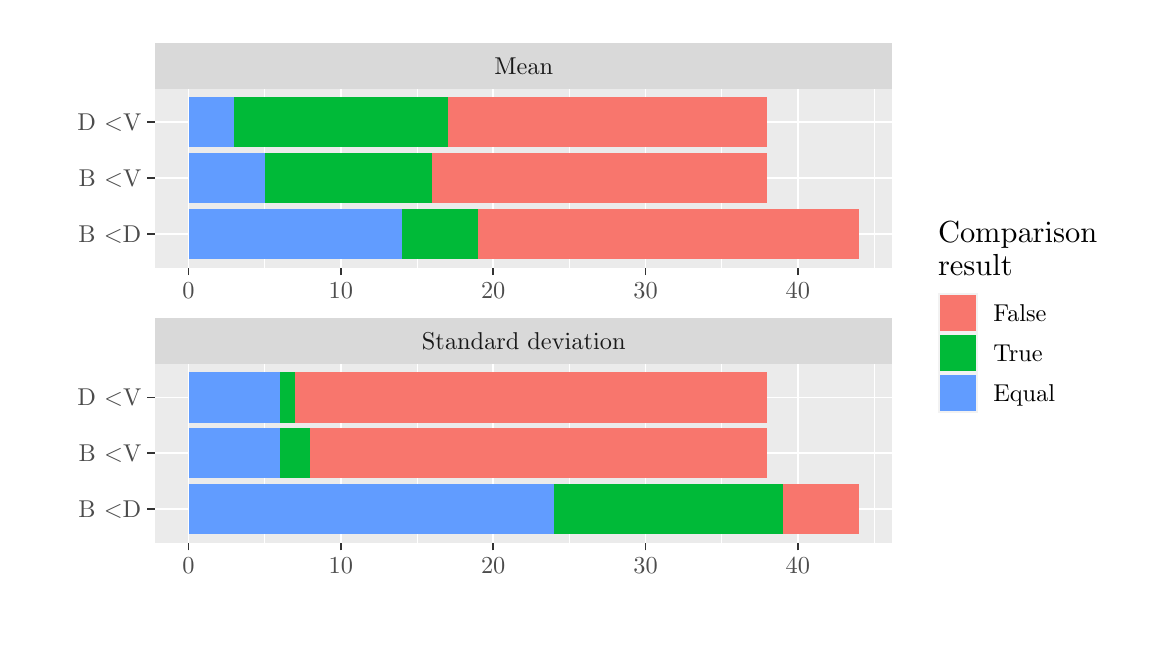
\begin{tikzpicture}[x=1pt,y=1pt]
\definecolor{fillColor}{RGB}{255,255,255}
\path[use as bounding box,fill=fillColor,fill opacity=0.00] (0,0) rectangle (397.48,216.81);
\begin{scope}
\path[clip] (  0.00,  0.00) rectangle (397.48,216.81);
\definecolor{drawColor}{RGB}{255,255,255}
\definecolor{fillColor}{RGB}{255,255,255}

\path[draw=drawColor,line width= 0.6pt,line join=round,line cap=round,fill=fillColor] (  0.00,  0.00) rectangle (397.48,216.81);
\end{scope}
\begin{scope}
\path[clip] ( 46.01,130.11) rectangle (312.46,194.74);
\definecolor{fillColor}{gray}{0.92}

\path[fill=fillColor] ( 46.01,130.11) rectangle (312.46,194.74);
\definecolor{drawColor}{RGB}{255,255,255}

\path[draw=drawColor,line width= 0.3pt,line join=round] ( 85.65,130.11) --
	( 85.65,194.74);

\path[draw=drawColor,line width= 0.3pt,line join=round] (140.70,130.11) --
	(140.70,194.74);

\path[draw=drawColor,line width= 0.3pt,line join=round] (195.75,130.11) --
	(195.75,194.74);

\path[draw=drawColor,line width= 0.3pt,line join=round] (250.80,130.11) --
	(250.80,194.74);

\path[draw=drawColor,line width= 0.3pt,line join=round] (305.86,130.11) --
	(305.86,194.74);

\path[draw=drawColor,line width= 0.6pt,line join=round] ( 46.01,142.23) --
	(312.46,142.23);

\path[draw=drawColor,line width= 0.6pt,line join=round] ( 46.01,162.42) --
	(312.46,162.42);

\path[draw=drawColor,line width= 0.6pt,line join=round] ( 46.01,182.62) --
	(312.46,182.62);

\path[draw=drawColor,line width= 0.6pt,line join=round] ( 58.12,130.11) --
	( 58.12,194.74);

\path[draw=drawColor,line width= 0.6pt,line join=round] (113.17,130.11) --
	(113.17,194.74);

\path[draw=drawColor,line width= 0.6pt,line join=round] (168.23,130.11) --
	(168.23,194.74);

\path[draw=drawColor,line width= 0.6pt,line join=round] (223.28,130.11) --
	(223.28,194.74);

\path[draw=drawColor,line width= 0.6pt,line join=round] (278.33,130.11) --
	(278.33,194.74);
\definecolor{fillColor}{RGB}{248,118,109}

\path[fill=fillColor] (162.72,133.14) rectangle (300.35,151.32);
\definecolor{fillColor}{RGB}{0,186,56}

\path[fill=fillColor] (135.19,133.14) rectangle (162.72,151.32);
\definecolor{fillColor}{RGB}{97,156,255}

\path[fill=fillColor] ( 58.12,133.14) rectangle (135.19,151.32);
\definecolor{fillColor}{RGB}{248,118,109}

\path[fill=fillColor] (146.20,153.34) rectangle (267.32,171.51);
\definecolor{fillColor}{RGB}{0,186,56}

\path[fill=fillColor] ( 85.65,153.34) rectangle (146.20,171.51);
\definecolor{fillColor}{RGB}{97,156,255}

\path[fill=fillColor] ( 58.12,153.34) rectangle ( 85.65,171.51);
\definecolor{fillColor}{RGB}{248,118,109}

\path[fill=fillColor] (151.71,173.53) rectangle (267.32,191.71);
\definecolor{fillColor}{RGB}{0,186,56}

\path[fill=fillColor] ( 74.64,173.53) rectangle (151.71,191.71);
\definecolor{fillColor}{RGB}{97,156,255}

\path[fill=fillColor] ( 58.12,173.53) rectangle ( 74.64,191.71);
\end{scope}
\begin{scope}
\path[clip] ( 46.01, 30.69) rectangle (312.46, 95.32);
\definecolor{fillColor}{gray}{0.92}

\path[fill=fillColor] ( 46.01, 30.69) rectangle (312.46, 95.32);
\definecolor{drawColor}{RGB}{255,255,255}

\path[draw=drawColor,line width= 0.3pt,line join=round] ( 85.65, 30.69) --
	( 85.65, 95.32);

\path[draw=drawColor,line width= 0.3pt,line join=round] (140.70, 30.69) --
	(140.70, 95.32);

\path[draw=drawColor,line width= 0.3pt,line join=round] (195.75, 30.69) --
	(195.75, 95.32);

\path[draw=drawColor,line width= 0.3pt,line join=round] (250.80, 30.69) --
	(250.80, 95.32);

\path[draw=drawColor,line width= 0.3pt,line join=round] (305.86, 30.69) --
	(305.86, 95.32);

\path[draw=drawColor,line width= 0.6pt,line join=round] ( 46.01, 42.80) --
	(312.46, 42.80);

\path[draw=drawColor,line width= 0.6pt,line join=round] ( 46.01, 63.00) --
	(312.46, 63.00);

\path[draw=drawColor,line width= 0.6pt,line join=round] ( 46.01, 83.20) --
	(312.46, 83.20);

\path[draw=drawColor,line width= 0.6pt,line join=round] ( 58.12, 30.69) --
	( 58.12, 95.32);

\path[draw=drawColor,line width= 0.6pt,line join=round] (113.17, 30.69) --
	(113.17, 95.32);

\path[draw=drawColor,line width= 0.6pt,line join=round] (168.23, 30.69) --
	(168.23, 95.32);

\path[draw=drawColor,line width= 0.6pt,line join=round] (223.28, 30.69) --
	(223.28, 95.32);

\path[draw=drawColor,line width= 0.6pt,line join=round] (278.33, 30.69) --
	(278.33, 95.32);
\definecolor{fillColor}{RGB}{248,118,109}

\path[fill=fillColor] (272.82, 33.72) rectangle (300.35, 51.89);
\definecolor{fillColor}{RGB}{0,186,56}

\path[fill=fillColor] (190.25, 33.72) rectangle (272.82, 51.89);
\definecolor{fillColor}{RGB}{97,156,255}

\path[fill=fillColor] ( 58.12, 33.72) rectangle (190.25, 51.89);
\definecolor{fillColor}{RGB}{248,118,109}

\path[fill=fillColor] (102.16, 53.91) rectangle (267.32, 72.09);
\definecolor{fillColor}{RGB}{0,186,56}

\path[fill=fillColor] ( 91.15, 53.91) rectangle (102.16, 72.09);
\definecolor{fillColor}{RGB}{97,156,255}

\path[fill=fillColor] ( 58.12, 53.91) rectangle ( 91.15, 72.09);
\definecolor{fillColor}{RGB}{248,118,109}

\path[fill=fillColor] ( 96.66, 74.11) rectangle (267.32, 92.29);
\definecolor{fillColor}{RGB}{0,186,56}

\path[fill=fillColor] ( 91.15, 74.11) rectangle ( 96.66, 92.29);
\definecolor{fillColor}{RGB}{97,156,255}

\path[fill=fillColor] ( 58.12, 74.11) rectangle ( 91.15, 92.29);
\end{scope}
\begin{scope}
\path[clip] ( 46.01, 95.32) rectangle (312.46,111.89);
\definecolor{fillColor}{gray}{0.85}

\path[fill=fillColor] ( 46.01, 95.32) rectangle (312.46,111.89);
\definecolor{drawColor}{gray}{0.10}

\node[text=drawColor,anchor=base,inner sep=0pt, outer sep=0pt, scale=  0.88] at (179.24,100.57) {Standard deviation};
\end{scope}
\begin{scope}
\path[clip] ( 46.01,194.74) rectangle (312.46,211.31);
\definecolor{fillColor}{gray}{0.85}

\path[fill=fillColor] ( 46.01,194.74) rectangle (312.46,211.31);
\definecolor{drawColor}{gray}{0.10}

\node[text=drawColor,anchor=base,inner sep=0pt, outer sep=0pt, scale=  0.88] at (179.24,199.99) {Mean};
\end{scope}
\begin{scope}
\path[clip] (  0.00,  0.00) rectangle (397.48,216.81);
\definecolor{drawColor}{gray}{0.20}

\path[draw=drawColor,line width= 0.6pt,line join=round] ( 58.12, 27.94) --
	( 58.12, 30.69);

\path[draw=drawColor,line width= 0.6pt,line join=round] (113.17, 27.94) --
	(113.17, 30.69);

\path[draw=drawColor,line width= 0.6pt,line join=round] (168.23, 27.94) --
	(168.23, 30.69);

\path[draw=drawColor,line width= 0.6pt,line join=round] (223.28, 27.94) --
	(223.28, 30.69);

\path[draw=drawColor,line width= 0.6pt,line join=round] (278.33, 27.94) --
	(278.33, 30.69);
\end{scope}
\begin{scope}
\path[clip] (  0.00,  0.00) rectangle (397.48,216.81);
\definecolor{drawColor}{gray}{0.30}

\node[text=drawColor,anchor=base,inner sep=0pt, outer sep=0pt, scale=  0.88] at ( 58.12, 19.68) {0};

\node[text=drawColor,anchor=base,inner sep=0pt, outer sep=0pt, scale=  0.88] at (113.17, 19.68) {10};

\node[text=drawColor,anchor=base,inner sep=0pt, outer sep=0pt, scale=  0.88] at (168.23, 19.68) {20};

\node[text=drawColor,anchor=base,inner sep=0pt, outer sep=0pt, scale=  0.88] at (223.28, 19.68) {30};

\node[text=drawColor,anchor=base,inner sep=0pt, outer sep=0pt, scale=  0.88] at (278.33, 19.68) {40};
\end{scope}
\begin{scope}
\path[clip] (  0.00,  0.00) rectangle (397.48,216.81);
\definecolor{drawColor}{gray}{0.20}

\path[draw=drawColor,line width= 0.6pt,line join=round] ( 58.12,127.36) --
	( 58.12,130.11);

\path[draw=drawColor,line width= 0.6pt,line join=round] (113.17,127.36) --
	(113.17,130.11);

\path[draw=drawColor,line width= 0.6pt,line join=round] (168.23,127.36) --
	(168.23,130.11);

\path[draw=drawColor,line width= 0.6pt,line join=round] (223.28,127.36) --
	(223.28,130.11);

\path[draw=drawColor,line width= 0.6pt,line join=round] (278.33,127.36) --
	(278.33,130.11);
\end{scope}
\begin{scope}
\path[clip] (  0.00,  0.00) rectangle (397.48,216.81);
\definecolor{drawColor}{gray}{0.30}

\node[text=drawColor,anchor=base,inner sep=0pt, outer sep=0pt, scale=  0.88] at ( 58.12,119.10) {0};

\node[text=drawColor,anchor=base,inner sep=0pt, outer sep=0pt, scale=  0.88] at (113.17,119.10) {10};

\node[text=drawColor,anchor=base,inner sep=0pt, outer sep=0pt, scale=  0.88] at (168.23,119.10) {20};

\node[text=drawColor,anchor=base,inner sep=0pt, outer sep=0pt, scale=  0.88] at (223.28,119.10) {30};

\node[text=drawColor,anchor=base,inner sep=0pt, outer sep=0pt, scale=  0.88] at (278.33,119.10) {40};
\end{scope}
\begin{scope}
\path[clip] (  0.00,  0.00) rectangle (397.48,216.81);
\definecolor{drawColor}{gray}{0.30}

\node[text=drawColor,anchor=base east,inner sep=0pt, outer sep=0pt, scale=  0.88] at ( 41.06,139.20) {B \textless D};

\node[text=drawColor,anchor=base east,inner sep=0pt, outer sep=0pt, scale=  0.88] at ( 41.06,159.39) {B \textless V};

\node[text=drawColor,anchor=base east,inner sep=0pt, outer sep=0pt, scale=  0.88] at ( 41.06,179.59) {D \textless V};
\end{scope}
\begin{scope}
\path[clip] (  0.00,  0.00) rectangle (397.48,216.81);
\definecolor{drawColor}{gray}{0.20}

\path[draw=drawColor,line width= 0.6pt,line join=round] ( 43.26,142.23) --
	( 46.01,142.23);

\path[draw=drawColor,line width= 0.6pt,line join=round] ( 43.26,162.42) --
	( 46.01,162.42);

\path[draw=drawColor,line width= 0.6pt,line join=round] ( 43.26,182.62) --
	( 46.01,182.62);
\end{scope}
\begin{scope}
\path[clip] (  0.00,  0.00) rectangle (397.48,216.81);
\definecolor{drawColor}{gray}{0.30}

\node[text=drawColor,anchor=base east,inner sep=0pt, outer sep=0pt, scale=  0.88] at ( 41.06, 39.77) {B \textless D};

\node[text=drawColor,anchor=base east,inner sep=0pt, outer sep=0pt, scale=  0.88] at ( 41.06, 59.97) {B \textless V};

\node[text=drawColor,anchor=base east,inner sep=0pt, outer sep=0pt, scale=  0.88] at ( 41.06, 80.17) {D \textless V};
\end{scope}
\begin{scope}
\path[clip] (  0.00,  0.00) rectangle (397.48,216.81);
\definecolor{drawColor}{gray}{0.20}

\path[draw=drawColor,line width= 0.6pt,line join=round] ( 43.26, 42.80) --
	( 46.01, 42.80);

\path[draw=drawColor,line width= 0.6pt,line join=round] ( 43.26, 63.00) --
	( 46.01, 63.00);

\path[draw=drawColor,line width= 0.6pt,line join=round] ( 43.26, 83.20) --
	( 46.01, 83.20);
\end{scope}
\begin{scope}
\path[clip] (  0.00,  0.00) rectangle (397.48,216.81);
\definecolor{fillColor}{RGB}{255,255,255}

\path[fill=fillColor] (323.46, 71.98) rectangle (391.98,153.44);
\end{scope}
\begin{scope}
\path[clip] (  0.00,  0.00) rectangle (397.48,216.81);
\definecolor{drawColor}{RGB}{0,0,0}

\node[text=drawColor,anchor=base west,inner sep=0pt, outer sep=0pt, scale=  1.10] at (328.96,139.30) {Comparison};

\node[text=drawColor,anchor=base west,inner sep=0pt, outer sep=0pt, scale=  1.10] at (328.96,127.42) {result};
\end{scope}
\begin{scope}
\path[clip] (  0.00,  0.00) rectangle (397.48,216.81);
\definecolor{fillColor}{gray}{0.95}

\path[fill=fillColor] (328.96,106.39) rectangle (343.42,120.85);
\end{scope}
\begin{scope}
\path[clip] (  0.00,  0.00) rectangle (397.48,216.81);
\definecolor{fillColor}{RGB}{248,118,109}

\path[fill=fillColor] (329.67,107.10) rectangle (342.71,120.13);
\end{scope}
\begin{scope}
\path[clip] (  0.00,  0.00) rectangle (397.48,216.81);
\definecolor{fillColor}{gray}{0.95}

\path[fill=fillColor] (328.96, 91.94) rectangle (343.42,106.39);
\end{scope}
\begin{scope}
\path[clip] (  0.00,  0.00) rectangle (397.48,216.81);
\definecolor{fillColor}{RGB}{0,186,56}

\path[fill=fillColor] (329.67, 92.65) rectangle (342.71,105.68);
\end{scope}
\begin{scope}
\path[clip] (  0.00,  0.00) rectangle (397.48,216.81);
\definecolor{fillColor}{gray}{0.95}

\path[fill=fillColor] (328.96, 77.48) rectangle (343.42, 91.94);
\end{scope}
\begin{scope}
\path[clip] (  0.00,  0.00) rectangle (397.48,216.81);
\definecolor{fillColor}{RGB}{97,156,255}

\path[fill=fillColor] (329.67, 78.20) rectangle (342.71, 91.23);
\end{scope}
\begin{scope}
\path[clip] (  0.00,  0.00) rectangle (397.48,216.81);
\definecolor{drawColor}{RGB}{0,0,0}

\node[text=drawColor,anchor=base west,inner sep=0pt, outer sep=0pt, scale=  0.88] at (348.92,110.59) {False};
\end{scope}
\begin{scope}
\path[clip] (  0.00,  0.00) rectangle (397.48,216.81);
\definecolor{drawColor}{RGB}{0,0,0}

\node[text=drawColor,anchor=base west,inner sep=0pt, outer sep=0pt, scale=  0.88] at (348.92, 96.13) {True};
\end{scope}
\begin{scope}
\path[clip] (  0.00,  0.00) rectangle (397.48,216.81);
\definecolor{drawColor}{RGB}{0,0,0}

\node[text=drawColor,anchor=base west,inner sep=0pt, outer sep=0pt, scale=  0.88] at (348.92, 81.68) {Equal};
\end{scope}
\end{tikzpicture}
